%\chapter{The Optimum Receiver}

\subsection{Breadboard}
The breadboard can be divided into 5 segments.  In each of the green segements, the pins are internally connected so as to have the same voltage.  Similarly, in the central segments, the pins in each column  are internally connected in the same fashion as the blue columns. 
\begin{figure}
\begin{center}
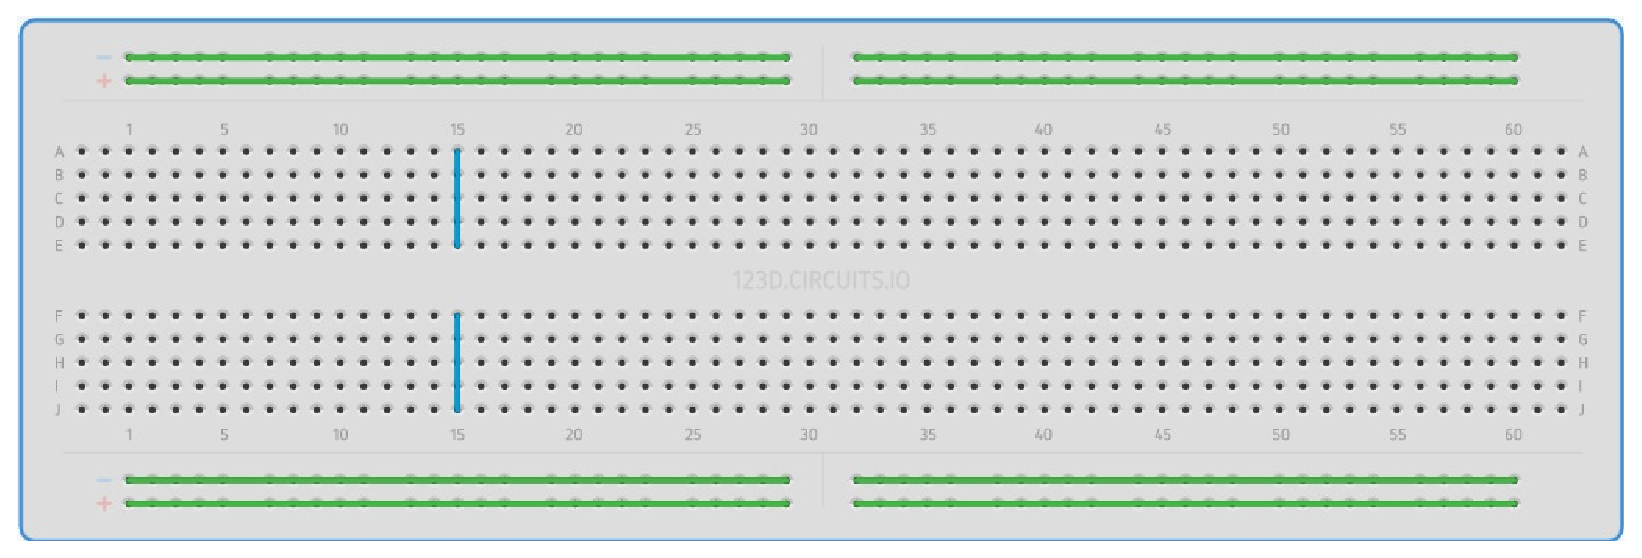
\includegraphics[width=\columnwidth]{breadboard}
\end{center}
\caption{}
\label{fig:breadboard}
\end{figure}



\subsection{Seven Segment Display}
The seven segment display has eight pins, $a, b, c, d, e, f, g$ and $dot$ that take an active LOW input, i.e.  the LED will glow only if the input is connected to ground.  Each of these pins is connected to an LED segment.  The $dot$ pin is  reserved for the $\cdot$ LED.  
%
\begin{figure}
\begin{center}
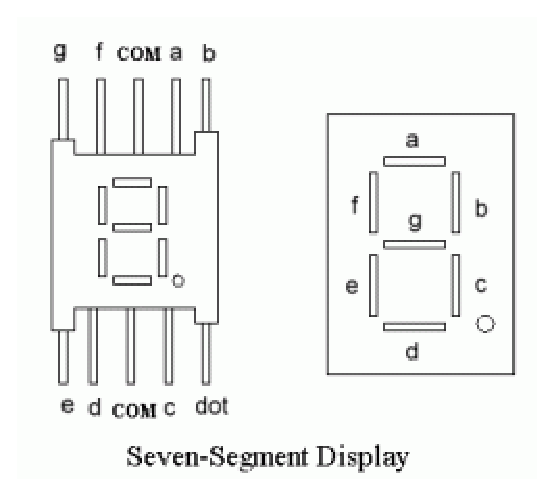
\includegraphics[width=\columnwidth]{sevenseg}
\end{center}
\caption{}
\label{fig:sevenseg}
\end{figure}

\subsection{Arduino}

The Arduino Uno has some ground pins, analog input pins A0-A3 and digital pins D1-D13 that can be used for both input as well as output. It also has two power pins that can generate 3.3$V$ and 5$V$.  In the following exercises, only the GND, 5$V$ and digital pins will be used.
%
\begin{figure}
\begin{center}
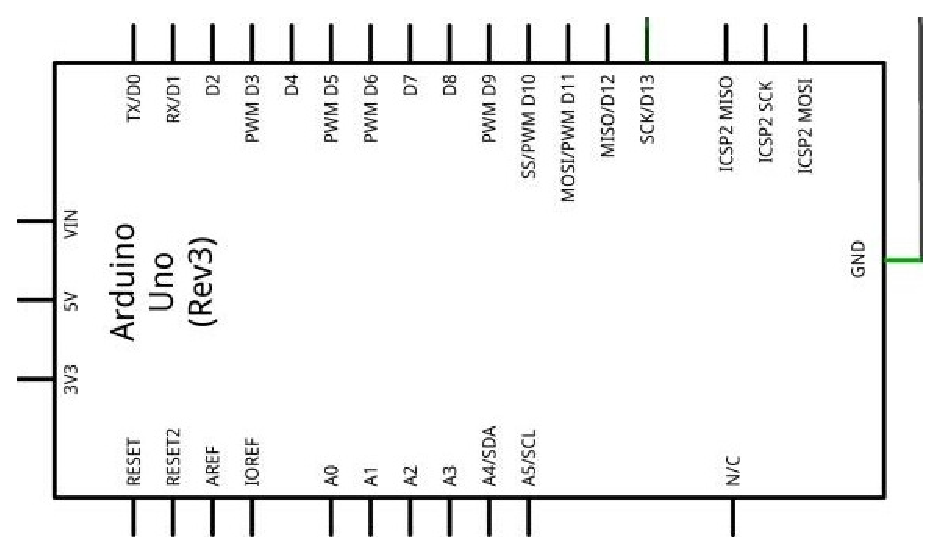
\includegraphics[width=\columnwidth]{arduino}
\end{center}
\caption{}
\label{fig:arduino}
\end{figure}

%\begin{center}
	%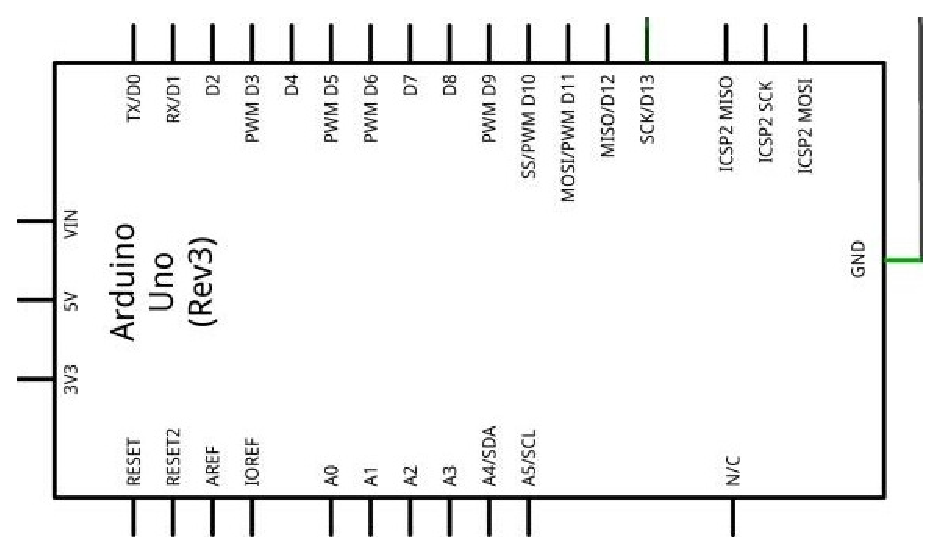
\includegraphics[scale=1]{arduino}
%\end{center}

\subsection{7447 Decoder}

The 7447 IC helps in displaying decimal numbers on the seven segment display.  The $\bar{a}-\bar{f}$, pins of the 7447 IC are connected to the $a-f$ pins of the display. $V_cc$ should be connected to a 5V power source. The input pins of the decoder are A,B,C and D, with A being the lowest significant bit (LSB) and D being the most significant bit (MSB).  For example, the number 5 is visible on the display when the A,B,C and D inputs are the following.
\begin{center}
	\begin{tabular}{|c|c|c|c|c|}
\hline
D & C & B & A & Decimal
\\ \hline
0 & 1 & 0 & 1 & 5
\\
\hline
\end{tabular}
\end{center}
%
%
\begin{figure}
\begin{center}
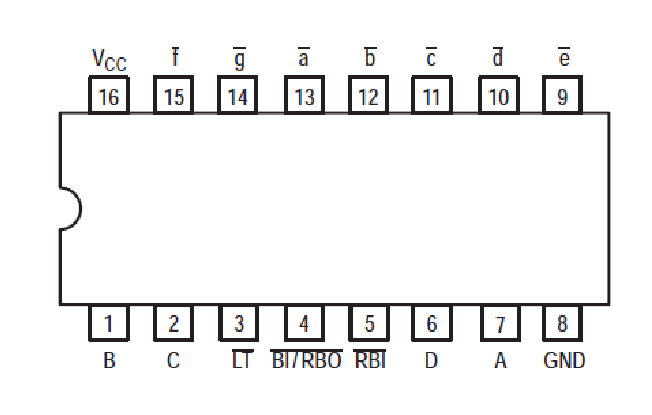
\includegraphics[width=\columnwidth]{7447IC}
\end{center}
\caption{}
\label{fig:7447IC}
\end{figure}

%\begin{center}
	%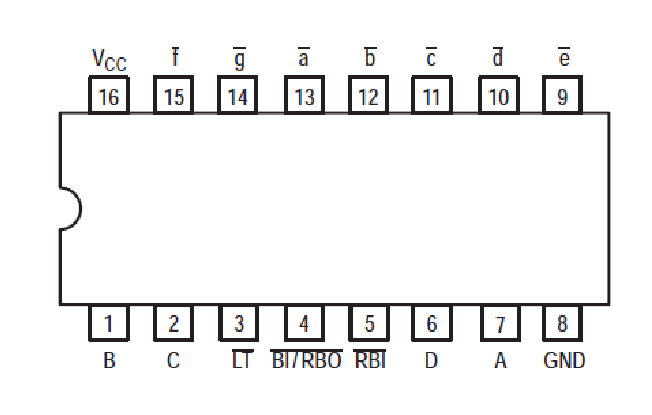
\includegraphics[scale=1.5]{7447IC}
%\end{center}


\subsection{7474 Flip Flop}
The 7474 IC has two flip flops.  The D pins denote the input and the Q pins denote the output. CLK denotes the clock input.
%
%
\begin{figure}
\begin{center}
\includegraphics[width=\columnwidth]{7474IC}
\end{center}
\caption{}
\label{fig:7474IC}
\end{figure}

%\begin{center}
	%\includegraphics[scale=1]{7474IC}
%\end{center}
